% !TeX spellcheck = en_US


\chapter{Experimental Setup}

To validate the proposed policies, we developed a framework comprising a simulation, tools for collecting metrics, and an automatic test runner.
It is based on the Mujoco physics engine, created by Google DeepMind, which provides a realistic simulation of contact dynamics.
The project is available on GitHub\footnote{\url{...}}.


\section{Swiping Policy} \label{sec:swiping-policy}

For the swiping policy, a single whisker executes a sweeping motion over the object.
Performance is quantified by evaluating the mean absolute error and the standard error in contour reconstruction, with each estimated point $\mathbf{y}_i$ matched to its closest reference point $\mathbf{x}_i$.

The estimated contour, $C_{\text{est}} = \{\mathbf{y}_i\}_{i=1}^N$, is determined by the control algorithm, which selects points based on whisker deflection and excludes those recorded during the whisking-back phase in retrieval.
The reference contour, $C_{\text{ref}} = \{\mathbf{x}_i\}_{i=1}^N$, consists of points on the object's surface, each being the closest match to the corresponding estimated point, and is derived from high-resolution sampling to serve as ground truth.

The absolute error is defined as $d_i = \|\mathbf{x}_i - \mathbf{y}_i\|$, which is the Euclidean distance between the reference and estimated points.
To assess performance, we compute the mean absolute error
\[
    \bar{d} = \frac{1}{N}\sum_{i=1}^{N} d_i,
\]
and the standard error
\[
    \sigma_d = \sqrt{\frac{1}{N-1}\sum_{i=1}^{N} (d_i - \bar{d})^2}.
\]
The mean absolute error represents the average distance between the reference and estimated points.

Figures~\ref{fig:experiment-disk-swiping}--\ref{fig:experiment-complex-object-swiping} display results for various objects.
Estimated contour points are colored green if their error deviates from the mean by less than the standard error, and red otherwise.
Red points indicate the most inaccurate measurements, corresponding to the worst 32 percentile of the error distribution.

\subsection{Contour Estimation of Disk and Rounded Rectangular Box}

Figure~\ref{fig:experiment-disk-swiping} shows the contour estimation of a disk using the swiping policy.
The disk is the simplest object, the mean reconstruction error is $0.8\,\text{mm} \pm 0.5\,\text{mm}$, indicating a high level of accuracy.
No prominent red regions are observed, except for occasional deviations due to the disk's polygonal approximation at the entry point.

\begin{figure}[!htb]
    \centering
    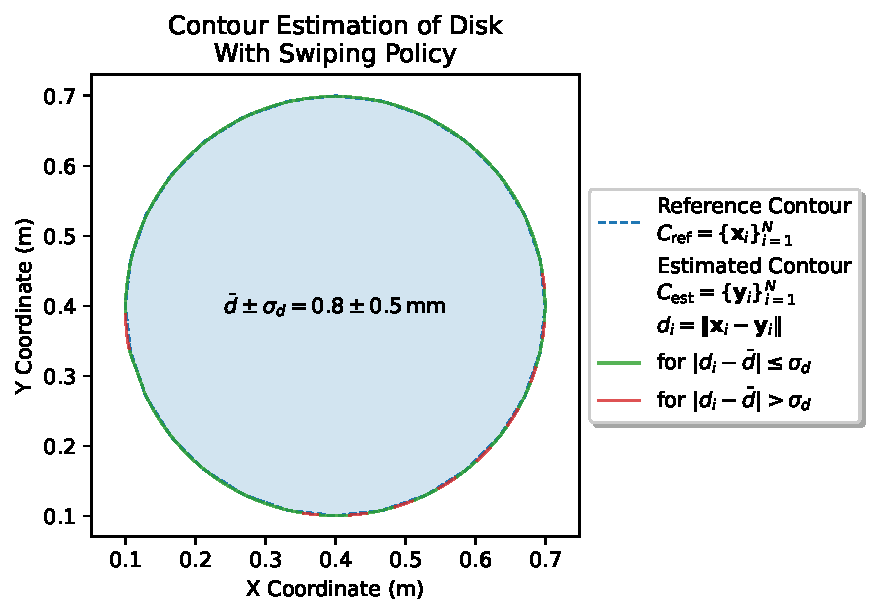
\includegraphics[width=0.8\textwidth]{figures/experiments/disk-swiping}
    \caption{Contour Estimation of Disk With Swiping Policy}
    \label{fig:experiment-disk-swiping}
\end{figure}

Figure~\ref{fig:experiment-rounded-rectangular-box-swiping} illustrates the contour estimation of a rounded rectangular box.
The rounded rectangular box is a more complex object with sharper corners, yet it shows a similar level of accuracy and mean error.
The mean reconstruction error is $0.8\,\text{mm} \pm 0.6\,\text{mm}$, with a single red region after the first corner.

\begin{figure}[!htb]
    \centering
    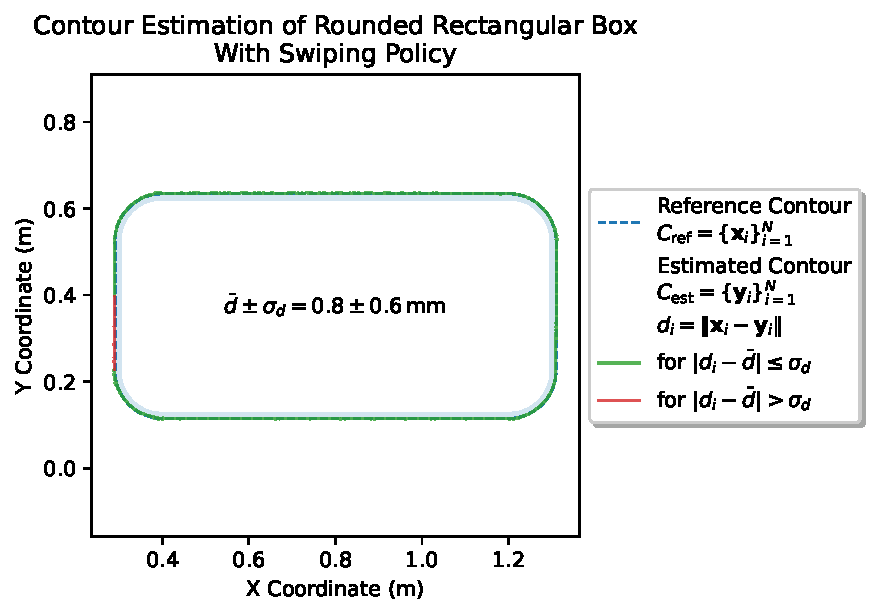
\includegraphics[width=0.8\textwidth]{figures/experiments/rounded-rectangular-box-swiping}
    \caption{Contour Estimation of Rounded Rectangular Box With Swiping Policy}
    \label{fig:experiment-rounded-rectangular-box-swiping}
\end{figure}

\subsection{Contour Estimation of Complex Object}

Figure~\ref{fig:experiment-complex-object-swiping} shows the contour estimation of a complex object.
Noticeable red regions appear at the inner inflections.
Since the inner angles are not smooth, the platform must quickly adjust to surface changes, which leads to a higher error rate.
At the initial moments, the whisker becomes overly deflected, causing the error to increase as the deflection model performs worse outside its normal operating range.
The mean error remains comparable to that observed for the disk and the rounded rectangular box.

Additionally, the swiping policy can successfully handle a 30\degree{} angle without causing the whisker to detach.
This angle is near the threshold where whisker detachment occurs and the retrieval policy is triggered.

\begin{figure}[!htb]
    \centering
    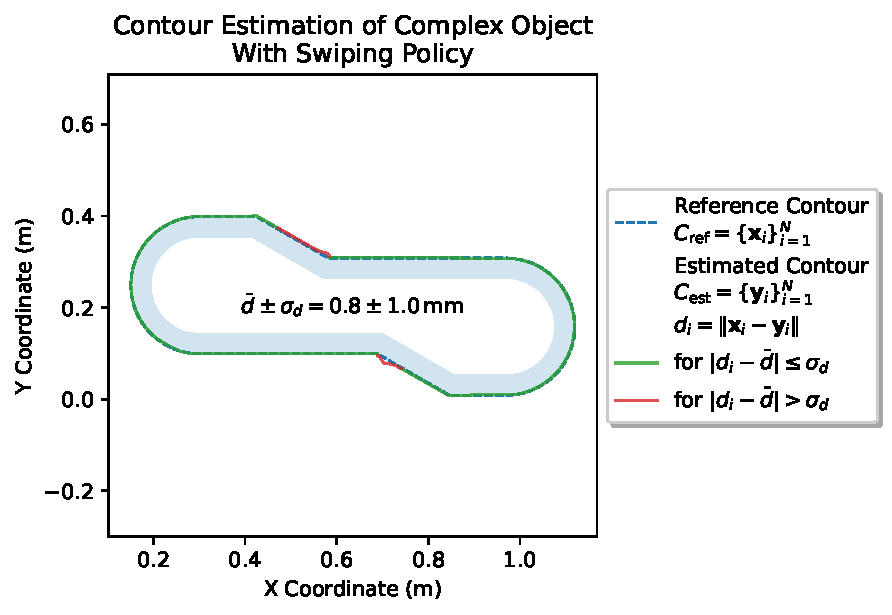
\includegraphics[width=0.8\textwidth]{figures/experiments/complex-object-swiping}
    \caption{Contour Estimation of Complex Object With Swiping Policy}
    \label{fig:experiment-complex-object-swiping}
\end{figure}


\section{Retrieval Policy}

Figures~\ref{fig:experiment-octagon-edges-135deg-swiping-retrieval}--\ref{fig:experiment-wall-edges-90deg-swiping-retrieval} show results for different polygonal objects.
Let $k_{\mathrm{edge}}$ be the index of an edge point and $k_{\mathrm{retr}}$ the index of its corresponding retrieved point, with the same indexing for both events.
The following metrics evaluate the retrieval policy:
\begin{itemize}
    \item \textbf{Mean absolute error:} $\bar{d} = \frac{1}{N}\sum_{i=1}^{N} d_i$, discussed in \cref{sec:swiping-policy}.
    \item \textbf{Mean retrieval radius:} $\bar{r} = \frac{1}{N}\sum_{j=1}^{N} \|\mathbf{r}_{\mathrm{edge},j} - \mathbf{r}_{\mathrm{retr},j}\|$, where $\mathbf{r}_{\mathrm{edge},j}$ is the $j$th edge point and $\mathbf{r}_{\mathrm{retr},j}$ its corresponding retrieved point.
    \item \textbf{Mean retrieval distance:} $\bar{d}_{\mathrm{retr}} = \frac{1}{N}\sum_{j=1}^{N}\sum_{i=i_{\mathrm{edge}_j}}^{i_{\mathrm{retr}_j}-1} \|\mathbf{r}^{t_{i+1}} - \mathbf{r}^{t_i}\|$, which calculates the trajectory length between the time of detachment and the time of retrieval, where $\mathbf{r}^{t}$ denotes the body position at time $t$.
\end{itemize}
In the plots, the edge points $\mathbf{r}_{\mathrm{edge}}$ are shown as red crosses, while the retrieved points $\mathbf{r}_{\mathrm{retr}}$ appear as black crosses.

The mean retrieval radius, defined as
\[
    \bar{r} = \frac{1}{N}\sum_{j=1}^{N} \|\mathbf{r}_{\mathrm{edge},j} - \mathbf{r}_{\mathrm{retr},j}\|,
\]
quantifies the proximity of a retrieved point to the edge, which is critical for accurately determining the edge direction.
A smaller $\bar{r}$ corresponds to a faster and more precise retrieval.
Ideally, this radius should be less than the distance between the whisker tip in its optimally deflected state (with $\delta=\delta_{\mathrm{target}}$) and its neutral state (with $\delta=0$), which is approximately 3\,cm.
The control algorithm sets the target mean retrieval radius to 1\,cm; values below 3\,cm are acceptable provided the contact angle remains within the desired range.

The mean retrieval distance, given by
\[
    \bar{d}_{\mathrm{retr}} = \frac{1}{N}\sum_{j=1}^{N}\sum_{i=k_{\mathrm{edge},j}}^{k_{\mathrm{retr},j}-1} \|\mathbf{r}^{t_{i+1}} - \mathbf{r}^{t_i}\|,
\]
measures the length of the trajectory from the time of detachment until the system resumes normal operation after retrieval.
A longer trajectory indicates more unnecessary movement, reducing the efficiency of the retrieval policy.
Note that for large, flat contact angles the whisker's overshoot may increase $\bar{r}$, even if the backward motion is not required to establish optimal contact.

The retrieval performance for the octagon with 135\degree{} edges is presented in Figure~\ref{fig:experiment-octagon-edges-135deg-swiping-retrieval}.
This object, with its high number of edges, demands a stable retrieval policy.
The octagon exhibits a mean reconstruction error of $1.1\,\text{mm} \pm 0.8\,\text{mm}$, comparable to the performance observed with the swiping policy.
It also has a mean retrieval radius of $20.9\,\text{mm} \pm 1.7\,\text{mm}$, which is about one quarter of the whisker length.
This radius is higher than the target of 1\,cm because fine adjustment of the whisker's position is unnecessary in this case.
The low relative standard deviation indicates high reproducibility.
The retrieval policy was triggered 8 times in total.

\begin{figure}[!htb]
    \centering
    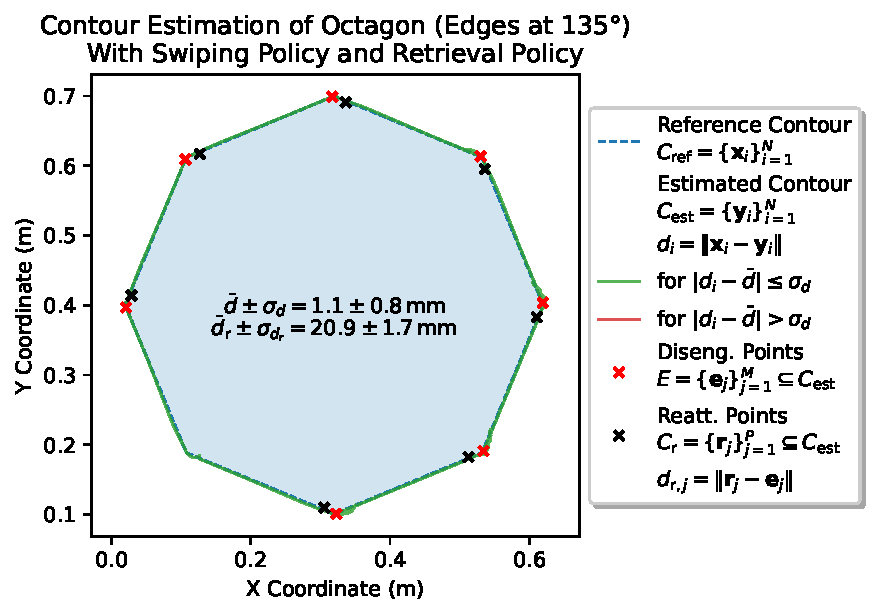
\includegraphics[width=0.8\textwidth]{figures/experiments/octagon-edges-135deg-swiping-retrieval}
    \caption{Contour Estimation of Octagon (Edges at 135°) With Swiping and Retrieval Policy}
    \label{fig:experiment-octagon-edges-135deg-swiping-retrieval}
\end{figure}

The retrieval on a box with 90\degree{} edges is shown in Figure~\ref{fig:experiment-box-edges-90deg-swiping-retrieval}.
The box’s sharper edges present a greater challenge for the whisker.
It achieves a mean reconstruction error of $0.7\,\text{mm} \pm 0.4\,\text{mm}$, demonstrating good performance.
It also has a mean retrieval radius of $11.2\,\text{mm} \pm 1.9\,\text{mm}$, which is close to the 1\,cm target while preserving retrieval consistency.

\begin{figure}[!htb]
    \centering
    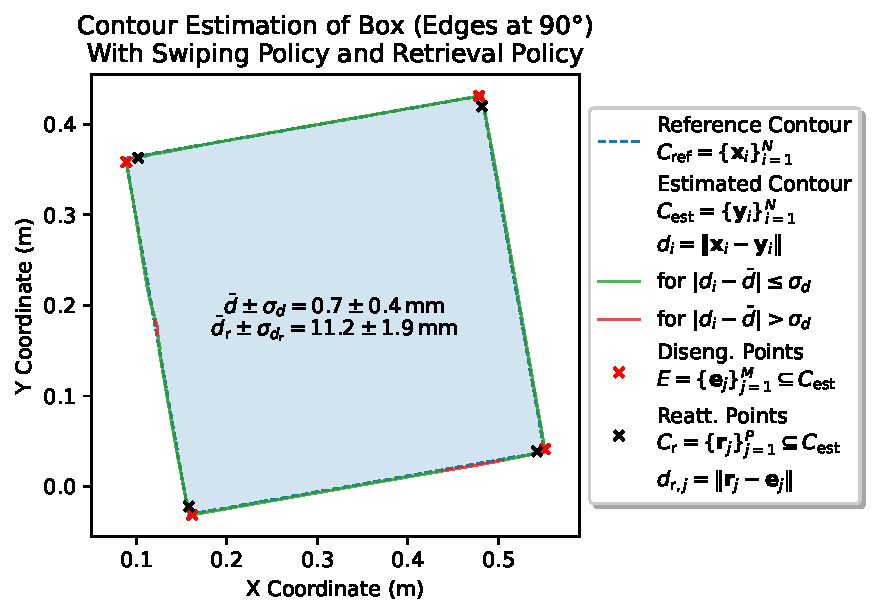
\includegraphics[width=0.8\textwidth]{figures/experiments/box-edges-90deg-swiping-retrieval}
    \caption{Contour Estimation of Box (Edges at 90°) With Swiping and Retrieval Policy}
    \label{fig:experiment-box-edges-90deg-swiping-retrieval}
\end{figure}

The performance on a prism with 60\degree{} edges is illustrated in Figure~\ref{fig:experiment-prism-edges-60deg-swiping-retrieval}.
The prism yields a mean reconstruction error of $0.8\,\text{mm} \pm 0.6\,\text{mm}$, in line with the swiping policy.
It also has a mean retrieval radius of $8.8\,\text{mm} \pm 0.6\,\text{mm}$, approaching the target value.
However, an inflation in the trajectory is observed at the retrieved edges.
This is likely due to the transition between the undeflected and deflected states.
Such overshoot—especially when the whisker contacts the edge away from its tip—is necessary to accelerate deflection compensation during subsequent swiping.
It also helps minimize the platform’s rocking in the normal direction.
A more sophisticated deflection model that accounts for contact along the whisker shaft could potentially mitigate this effect.

\begin{figure}[!htb]
    \centering
    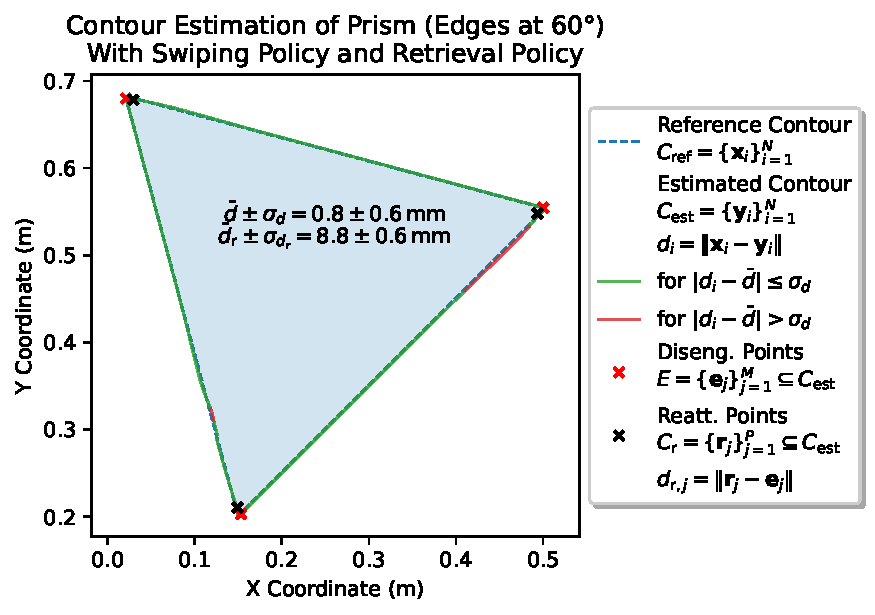
\includegraphics[width=0.8\textwidth]{figures/experiments/prism-edges-60deg-swiping-retrieval}
    \caption{Contour Estimation of Prism (Edges at 60°) With Swiping and Retrieval Policy}
    \label{fig:experiment-prism-edges-60deg-swiping-retrieval}
\end{figure}

The wall experiment with 90\degree{} edges is presented in Figure~\ref{fig:experiment-wall-edges-90deg-swiping-retrieval}.
This scenario is challenging because the wall’s width is only 1\,cm, matching the target retrieval radius.
Nonetheless, the system achieves a mean retrieval radius of $10.2\,\text{mm} \pm 0.7\,\text{mm}$, nearly meeting the target.
This performance is partly due to the wall’s precise 1\,cm width, which limits the possibility of contacts farther away.
Video recordings confirm that the whisker tip is well-aligned and contacts the opposite edge accurately.
If the wall were about 25\% shorter, the policy could still handle it through deflection at the whisker’s shaft, provided the side length remains above a critical threshold.
Conversely, when the target radius is doubled, the platform executes a 180\degree{} turn to reach the edge, effectively rendering the wall undetectable.
In this case, the mean reconstruction error is $1.1\,\text{mm} \pm 0.6\,\text{mm}$, consistent with the performance of the swiping policy.

\begin{figure}[!htb]
    \centering
    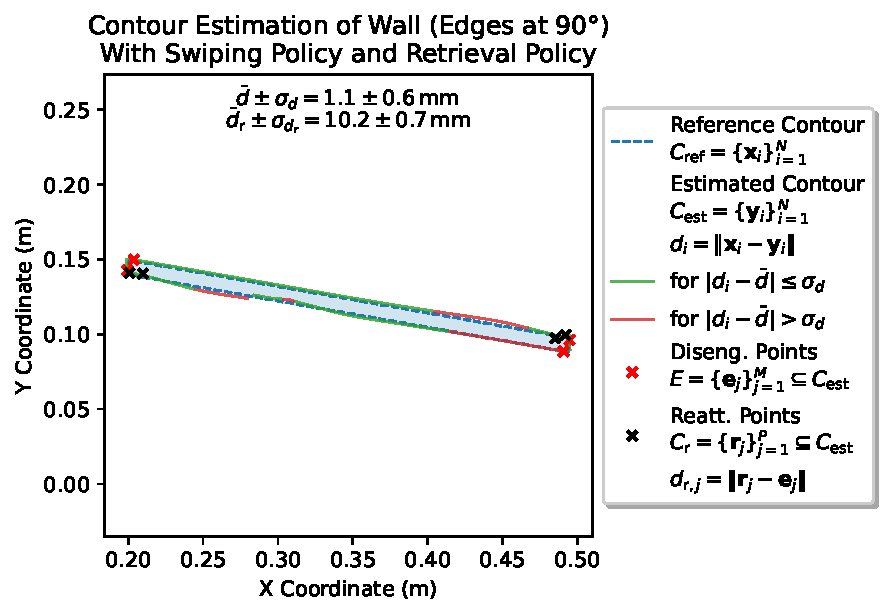
\includegraphics[width=0.8\textwidth]{figures/experiments/wall-edges-90deg-swiping-retrieval}
    \caption{Contour Estimation of Wall (Edges at 90°) With Swiping and Retrieval Policy}
    \label{fig:experiment-wall-edges-90deg-swiping-retrieval}
\end{figure}


\section{Tunneling Policy}
A tunneling policy extends the swiping policy to navigate confined environments.
Its goal is to maintain a centered trajectory in the tunnel to avoid collisions and ensure accurate contour estimation.

For the tunneling policy, we employ the following metrics:

\begin{itemize}
    \item \textbf{Mean absolute reconstruction error:}
    \[
        \bar{d} = \frac{1}{NK}\sum_{i=1}^{N}\sum_{k=1}^{K} d_{i,k},
    \]
    where
    \[
        d_{i,k} = \|\mathbf{x}_{i,k} - \mathbf{y}_{i,k}\|
    \]
    is the distance between the $i$th reference point $\mathbf{x}_{i,k}$ and the corresponding estimated point $\mathbf{y}_{i,k}$ of the $k$th whisker.
    \item \textbf{Mean absolute axis error:}
    \[
        \bar{d}_{\mathrm{axis}} = \frac{1}{N}\sum_{i=1}^{N} d_{\mathrm{axis},i},
    \]
    where
    \[
        d_{\mathrm{axis},i} = \|\mathbf{a}_i - \mathbf{a}_m\|
    \]
    is the distance between the point $\mathbf{a}_i$ on the tunnel axis closest to the $i$th estimated midpoint and the axis $\mathbf{a}_m$, with the estimated midpoint defined as
    \[
        \mathbf{m}_i = \frac{\mathbf{x}_{i,\mathrm{l}} + \mathbf{y}_{i,\mathrm{r}}}{2}.
    \]
\end{itemize}

The tunnel axis, shown as pink dashed lines in the figures, is defined as the line equidistant from the tunnel walls.
Thus, the mean absolute axis error quantifies the deviation of the estimated midpoints (marked in black) from the tunnel axis.

Figures~\ref{fig:experiment-smooth-tunnel-swiping-tunneling}--\ref{fig:experiment-round-tunnel-swiping-tunneling} illustrate smooth, zigzag, and round tunnels.

The smooth tunnel in Figure~\ref{fig:experiment-smooth-tunnel-swiping-tunneling} represents the simplest case.
The whisker successfully navigates the tunnel while maintaining a centered trajectory.
The mean absolute reconstruction error is $1.3\,\text{mm} \pm 1.6\,\text{mm}$, and the mean absolute axis error is $4\,\text{mm} \pm 4\,\text{mm}$.
For reference, the tunnel is approximately 10\,cm wide, and each whisker is 7.5\,cm long.
The difference between the reconstruction error and the axis error is due to a lag in the midpoint trajectory relative to the tunnel axis.
This lag occurs because the control system cannot immediately adjust the platform’s position owing to its inertia and the continuously changing tunnel direction.
Additionally, heightened deflection near the operational limit of the deflection model and a transition effect when the whiskers first contact the tunnel walls contribute to this error.

\begin{figure}[!htb]
    \centering
    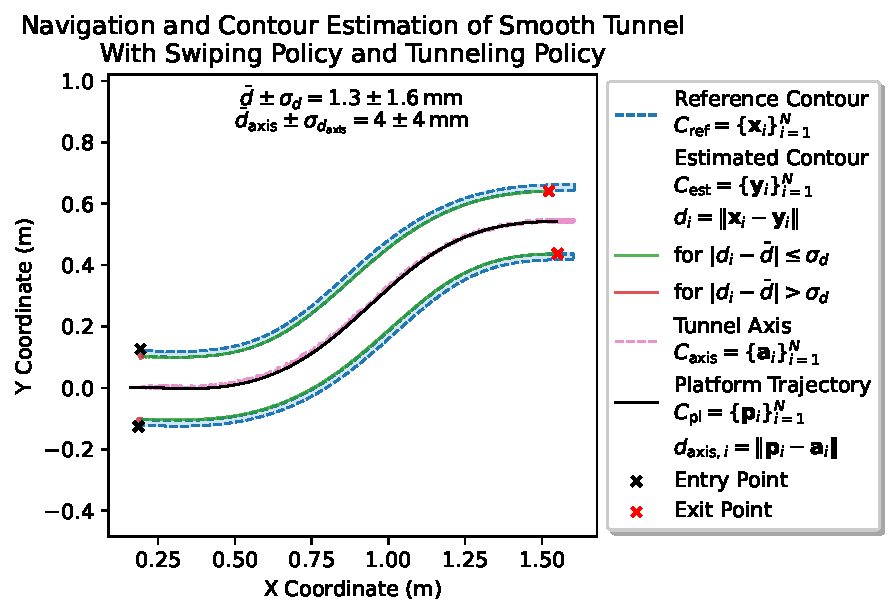
\includegraphics[width=0.8\textwidth]{figures/experiments/smooth-tunnel-swiping-tunneling}
    \caption{Navigation and Contour Estimation of Smooth Tunnel With Swiping and Tunneling Policy}
    \label{fig:experiment-smooth-tunnel-swiping-tunneling}
\end{figure}

The zigzag tunnel in Figure~\ref{fig:experiment-zigzag-tunnel-swiping-tunneling}, with angles of $20^\circ$ and $40^\circ$, is more complex due to its sharper corners.
In this case, the mean absolute reconstruction error is $2\,\text{mm} \pm 2\,\text{mm}$, while the mean absolute axis error increases to $9\,\text{mm} \pm 10\,\text{mm}$.
This increase is attributed to the difficulty of maintaining a centered trajectory, as the midpoint trajectory deviates from the tunnel axis at the corners.
Furthermore, the left whisker detaches at the first zigzag, while the right whisker remains in contact with the wall.
Because the left whisker cannot maintain contact at the sharp angle, the swiping policy is applied to the right whisker until the left whisker re-establishes contact.
For a short period, the platform’s nose contacts the wall, but it quickly recovers.
Overall, the performance is satisfactory, as the whiskers navigate the tunnel and accurately estimate the contour.
For even sharper zigzag angles, the platform may fail to pass through the tunnel if its nose prods a wall, as no recovery policy is implemented for such cases.
Such failures would be indicated by increased actuator force or a reduction in platform speed, which are not measured in the current setup.

\begin{figure}[!htb]
    \centering
    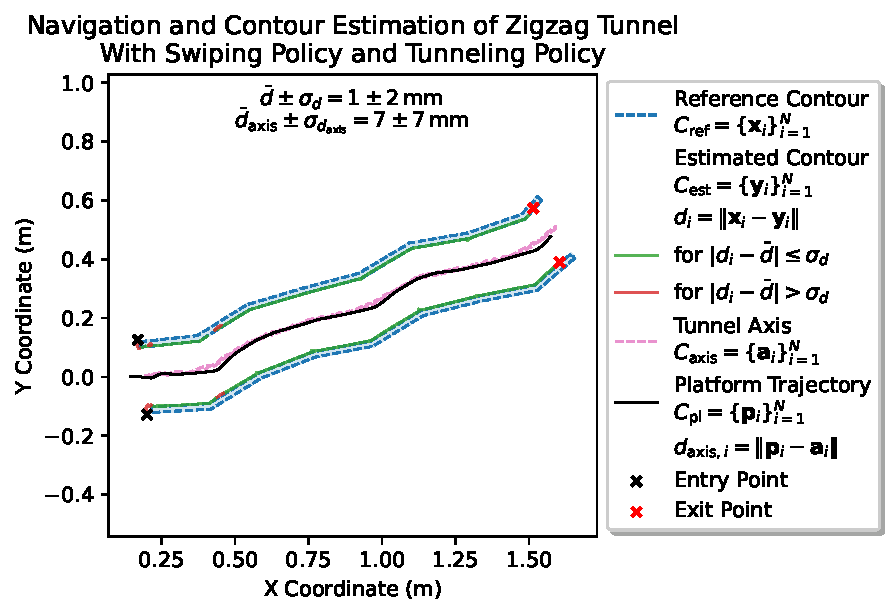
\includegraphics[width=0.8\textwidth]{figures/experiments/zigzag-tunnel-swiping-tunneling}
    \caption{Navigation and Contour Estimation of Zigzag Tunnel With Swiping and Tunneling Policy}
    \label{fig:experiment-zigzag-tunnel-swiping-tunneling}
\end{figure}

The round tunnel in Figure~\ref{fig:experiment-round-tunnel-swiping-tunneling} tests the endurance of the tunneling policy.
It involves a longer trajectory and a star-shaped loop.
A pronounced transition effect is observed at the start, as the whisker adjusts to the tunnel’s curvature and the initial position (marked by black crosses) is not aligned with the tunnel axis.
Skidding is also noticeable at the sharper curves.
The performance remains satisfactory, with a mean absolute reconstruction error of $3\,\text{mm} \pm 2\,\text{mm}$ and a mean absolute axis error of $5\,\text{mm} \pm 6\,\text{mm}$.
The increased reconstruction error is likely due to operating outside the optimal range of the deflection model at the curves.
This is evident in segments of the tunnel marked in red, where the outer whisker (right, in this case) experiences excessive compression.

\begin{figure}[!htb]
    \centering
    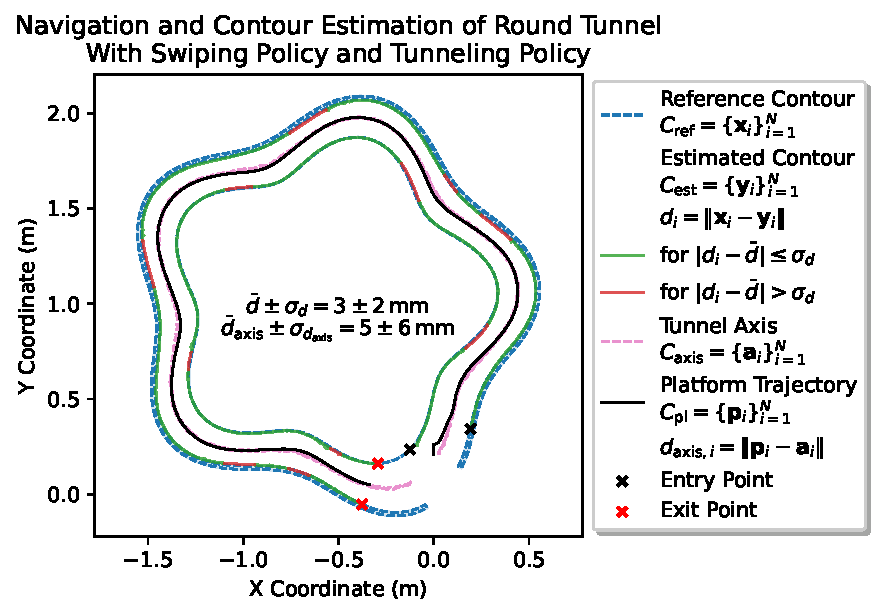
\includegraphics[width=0.8\textwidth]{figures/experiments/round-tunnel-swiping-tunneling}
    \caption{Navigation and Contour Estimation of Round Tunnel With Swiping and Tunneling Policy}
    \label{fig:experiment-round-tunnel-swiping-tunneling}
\end{figure}
